%% PX1 manuscript, Elsevier CAS single-column template (cas-sc), as used by the group's earlier submission.
%% Target: ISPRS Journal of Photogrammetry and Remote Sensing (first submission may be any format, "Your Paper Your Way").
%% Final draft, 10 Nov 2026.

\documentclass[a4paper,fleqn]{cas-sc}

\usepackage[numbers,sort&compress]{natbib}
\usepackage{booktabs}
\usepackage{multirow}
\usepackage{amsmath,amssymb}
\usepackage{xcolor}
\usepackage{siunitx}
\sisetup{detect-all}

\begin{document}
\let\WriteBookmarks\relax
\def\floatpagepagefraction{1}
\def\textpagefraction{.001}
\let\printorcid\relax

\shorttitle{Safe test-time adaptation for SAR flood mapping}
\shortauthors{M.S. Hasan et al.}

\title [mode = title]{Safe test-time adaptation for SAR flood mapping: physics-checked self-training with a flood-level miss-rate guarantee}

\author[1]{MD Sakib Hasan}
\author[1]{Mostofa Seum}
\author[1]{Meer Mursalin}
\author[1]{Tanvir Ahmed}[]
\cormark[1]
\ead{tanvir.ahmed@aiub.edu}
\author[1]{Rifath Mahmud}
\author[1]{Syeda Anika Tasnim}

\affiliation[1]{organization={Department of Computer Science, American International University-Bangladesh (AIUB)},
            addressline={408/1, Kuratoli, Khilkhet},
            city={Dhaka},
            postcode={1229},
            country={Bangladesh}}

\cortext[1]{Corresponding author}

\begin{abstract}
Deep networks trained to map floods in Sentinel-1 radar images lose much of their accuracy on floods unlike those they were trained on, and in an emergency there are no labels to retrain them. Test-time adaptation can update a model on the unlabelled images of a new flood, but it can also make the map worse, and a single default threshold says nothing about how much flood water the map misses. We propose a label-free adaptation that re-estimates batch-normalisation statistics on the new flood and then self-trains on pseudo-labels checked against radar and terrain physics: pixels that are dark in both polarisations (relative to a threshold derived from the flood's own backscatter histogram), lie less than 5\,m above the nearest drainage and are nearly flat are added as water. The flood-map threshold is then calibrated by conformal risk control with flood events, not pixels, as the exchangeable unit, so the average miss rate over new floods is bounded at a level chosen by the user. Models trained on Sen1Floods11 were evaluated leave-one-flood-out on Sen1Floods11, on 26 events of Kuro Siwo and, in a pre-registered final test, on 30 activations of MMFlood that played no part in any design decision. On Kuro Siwo the method reached an intersection over union (IoU) of 0.677 under a 20\% miss-rate guarantee, against 0.467 for TENT and 0.565 without adaptation. On MMFlood it beat TENT and batch-norm adaptation under the guarantee on 28 of 30 floods (Holm-corrected $p<10^{-7}$), and the mean miss rate stayed below the 20\% target (0.177), but it did not beat the unadapted model at the default threshold. Plain test-time adaptation lowered the accuracy of guaranteed maps on MMFlood; the physics check removed this harm. An ImageNet-pretrained ResNet-34 backbone, with and without additional training floods, reproduced the pattern on both test datasets, and the results changed little when the method's settings were varied.
\end{abstract}

%% Highlights are uploaded as a separate file (highlights.txt), as Elsevier asks.


\begin{keywords}
flood mapping \sep synthetic aperture radar \sep test-time adaptation \sep conformal prediction \sep height above nearest drainage \sep Sentinel-1
\end{keywords}

\maketitle

%% =====================================================================
\section{Introduction}
\label{sec:intro}

Floods affect more people than any other natural hazard, and the share of the world's population living in flood-exposed areas is rising \citep{tellman2021exposure}. Synthetic aperture radar (SAR) sees through clouds and at night, which makes Sentinel-1 \citep{torres2012sentinel1} the main source of rapid flood maps: open water reflects little radar energy back to the sensor and appears dark. Operational systems such as the Copernicus Global Flood Monitoring service combine thresholding, change detection and terrain masks \citep{salamon2021gfm,twele2016s1chain,zhao2021exclusion}, and deep networks trained on labelled benchmarks \citep{bonafilia2020sen1floods11,bountos2024kurosiwo,montello2022mmflood} now outperform thresholds on images like those they were trained on \citep{bentivoglio2022review,helleis2022benchmark}.

Two problems limit their use in an emergency. First, accuracy drops sharply on floods unlike the training data: different landscapes, seasons, radar calibration and labelling conventions \citep{bentivoglio2022review,turkmenli2025dgflood}. In our experiments, models trained on Sen1Floods11 missed 74\% of the flood water in Kuro Siwo at the default threshold. Labels for the new flood are not available in time to retrain. Test-time adaptation (TTA) updates a model on the unlabelled images it is asked to map, for example by re-estimating batch-normalisation statistics \citep{li2018adabn,schneider2020covariate}, minimising prediction entropy \citep{wang2021tent} or self-training on its own confident predictions \citep{tarvainen2017meanteacher,wang2022cotta}. \citet{chen2026cimttda} recently showed that pseudo-label self-training improves SAR inundation maps across coastal flood events. TTA can also fail, however, and a model can confirm and amplify its own mistakes \citep{niu2023sar}.

Second, a flood map is usually produced by thresholding a probability at 0.5, and nothing tells the user how much flooding the map misses. For emergency response, missed flood water is the costlier error. Deep networks are poorly calibrated \citep{guo2017calibration}, and calibration degrades further on new data. Heuristic uncertainty estimates exist for flood maps \citep{gal2016dropout,lakshminarayanan2017ensembles,chen2026uncertaintyflood}, but they do not bound an error rate. Conformal prediction gives distribution-free guarantees \citep{vovk2022alrw,angelopoulos2023gentle}, and conformal risk control can bound the expected false negative rate of a segmentation \citep{angelopoulos2024crc}. Its use for flood maps has so far been limited to pixel-level prediction sets on optical images without domain shift \citep{konidakis2025cpflood}.

This paper combines the two. Our hypothesis is that SAR flood physics, namely that open water is dark and lies low in flat terrain, provides an independent check on the pseudo-labels a model produces for itself, and that this check can make adaptation safe. The contributions are:
\begin{itemize}
\item A label-free test-time adaptation for SAR flood mapping that re-estimates batch-normalisation statistics and then self-trains on pseudo-labels corrected by a per-flood radar threshold, height above nearest drainage (HAND) \citep{renno2008hand,nobre2011hand} and slope.
\item A flood-level miss-rate guarantee: conformal risk control calibrated across flood events, so that the average fraction of missed flood water over new floods stays below a chosen level.
\item An evaluation on three datasets with events as the statistical unit, including a pre-registered final test on 30 MMFlood activations that were not used for any design decision \citep{nosek2018prereg}.
\item Evidence that plain TTA can lower the accuracy of guaranteed flood maps on a new dataset, and that the physics check removes this harm; the pattern holds for a second, ImageNet-pretrained backbone and for more diverse training data.
\end{itemize}

Section~\ref{sec:related} reviews related work, Section~\ref{sec:method} describes the method, Section~\ref{sec:setup} the data and experimental protocol, Section~\ref{sec:results} the results, and Section~\ref{sec:discussion} discusses them with their limitations.

%% =====================================================================
\section{Related work}
\label{sec:related}

\subsection{SAR flood mapping}
Classical SAR flood mapping thresholds backscatter, often per tile or with parametric fits \citep{otsu1979threshold,martinis2009nrt,chini2017hsbt}, uses change detection against a pre-flood image \citep{giustarini2013change,clement2018multitemporal}, and refines the result with terrain and context \citep{twele2016s1chain,landuyt2019assessment}. Probabilistic variants estimate per-pixel flood probabilities \citep{giustarini2016probabilistic,krullikowski2023gfmensemble}. Known failure modes are flooded vegetation and urban areas, where water is bright rather than dark \citep{tsyganskaya2018vegetation,zhao2024urbansarfloods}. Deep learning has become standard since public benchmarks appeared \citep{bonafilia2020sen1floods11,mateogarcia2021worldfloods,drakonakis2022ombrianet,bountos2024kurosiwo,montello2022mmflood}, with convolutional networks \citep{nemni2020unosat,bai2021basnet,konapala2021s1s2}, change-detection networks applied globally \citep{misra2025globalfloods} and geospatial foundation models \citep{jakubik2023prithvi}. Reviews identify generalisation to new floods and uncertainty as the main open problems \citep{bentivoglio2022review,lee2025geoaiflood}.

\subsection{Terrain priors}
HAND, the height of a pixel above the nearest drainage channel \citep{renno2008hand,nobre2011hand}, is widely used to rule out implausible flooding. It serves as a post-hoc mask or exclusion layer \citep{twele2016s1chain,zhao2021exclusion,misra2025globalfloods}, as a prior in Bayesian flood mapping \citep{tupas2023handprior}, as a network input \citep{tian2026deepsar} and in rule-based refinement \citep{hansen2025ribe}. Elevation can also shape the training loss \citep{sami2024evanet}. More broadly, physics-guided machine learning uses scientific knowledge to constrain data-driven models \citep{karpatne2017tgds,reichstein2019deep,willard2022integrating}. We use terrain and radar physics at a different point: to correct pseudo-labels during label-free adaptation on the target flood.

\subsection{Domain adaptation and test-time adaptation}
Domain shift is a long-standing problem in remote sensing \citep{tuia2016darsreview}. Unsupervised domain adaptation with self-training \citep{lee2013pseudolabel,zou2018cbst,hoyer2022daformer} needs the source data during adaptation. TTA adapts with target data only: AdaBN re-estimates batch-normalisation statistics \citep{li2018adabn,schneider2020covariate}, TENT minimises entropy \citep{wang2021tent}, teacher-student methods use pseudo-labels from an exponential-moving-average teacher \citep{tarvainen2017meanteacher,wang2022cotta}, and reliability filtering aims to avoid collapse \citep{niu2022eata,niu2023sar}; see \citet{liang2025ttasurvey} for a survey. TTA has been applied to remote-sensing segmentation and classification \citep{wang2024rsselfprompt,liang2024lscdtta} and to SAR coastal inundation \citep{chen2026cimttda}. For floods, label-efficient alternatives include adversarial adaptation with label refinement \citep{akiva2021h2onet}, semi-supervised pseudo-labelling \citep{paul2021semisup}, cross-modal distillation \citep{garg2023crossmodal}, unsupervised change detection on time series \citep{yadav2022unsupts} and domain generalisation across events \citep{turkmenli2025dgflood}. None of these checks pseudo-labels against physics or attaches a guarantee to the adapted map.

\subsection{Conformal prediction and risk control}
Conformal prediction produces distribution-free guarantees under exchangeability \citep{vovk2022alrw,lei2018distfree,angelopoulos2023gentle}. Risk-controlling prediction sets \citep{bates2021rcps}, conformal risk control \citep{angelopoulos2024crc} and learn-then-test \citep{angelopoulos2021ltt} extend it to general losses such as the false negative rate of a segmentation \citep{mossina2024conformalseg}. Under distribution shift the guarantee needs weighting or degrades gracefully \citep{tibshirani2019covshift,barber2023beyond}; when data come in groups, the groups rather than their members must be exchangeable \citep{dunn2023hierarchical}. In flood mapping, conformal methods have so far produced pixel-level prediction sets for optical images \citep{konidakis2025cpflood} and, for SAR, set out-of-distribution abstention and set-valued predictions \citep{li2026crcflood}; neither bounds the miss rate across flood events or is combined with test-time adaptation. We treat flood events as the exchangeable unit and calibrate leave-one-event-out.

%% =====================================================================
\section{Method}
\label{sec:method}
Fig.~\ref{fig:method} summarises the three steps applied to each new flood event.

\begin{figure}[t]
\centering
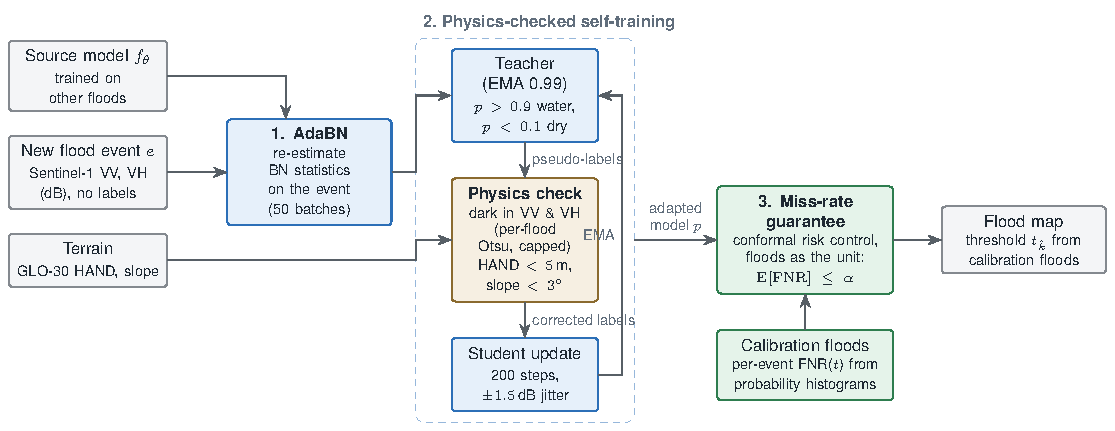
\includegraphics[width=\textwidth]{figures/fig_method.pdf}
\caption{Overview of the method. (1) AdaBN re-estimates batch-normalisation statistics on the unlabelled event. (2) A mean teacher produces confident pseudo-labels, which are corrected with a per-flood radar darkness test and HAND/slope limits before each student update. (3) The decision threshold is set by conformal risk control on other flood events, so that the expected per-flood miss rate stays below $\alpha$.}
\label{fig:method}
\end{figure}

\subsection{Problem setting}
A segmentation network $f_\theta$ is trained on labelled Sentinel-1 chips (VV and VH backscatter in dB) from a set of source floods. At test time it receives the chips $\mathcal{X}_e$ of a new flood event $e$, without labels, and must output a binary flood map. For each pixel $f_\theta$ gives a water probability $p$; the map is $\{p \ge t\}$ for a threshold $t$. We want (i) maps that are as accurate as possible on $e$ and (ii) a threshold whose expected miss rate (false negative rate, FNR) over new events is at most a user-chosen $\alpha$.

\subsection{Batch-normalisation re-estimation}
Radar calibration and land cover differ between datasets, which shifts the statistics of intermediate features. Following AdaBN \citep{li2018adabn}, we reset the running mean and variance of every batch-normalisation layer and re-estimate them as a cumulative average over 50 batches of eight random $256\times256$ crops (with random rotations and flips) of the event's chips. No weights are trained; this takes about 10\,s per event.

\subsection{Physics-checked self-training}
After AdaBN, a copy of the network serves as teacher and the network itself as student. For 200 steps, a batch of eight random crops is drawn from the event. The teacher's water probability $p$ gives a pseudo-label of water where $p>0.9$, dry where $p<0.1$, and no label otherwise. These pseudo-labels are then checked against physics:
\begin{itemize}
\item \textbf{Per-flood dark threshold.} For each polarisation, an Otsu threshold \citep{otsu1979threshold} is computed on the backscatter of all chips of the event, together with the mean $\mu_d$ of the darker class. The dark threshold is the midpoint between them, capped at $-15$\,dB (VV) and $-22$\,dB (VH) so that a flood with little open water cannot turn dry land into water. The rule was fixed before any of the reported runs.
\item \textbf{Low and flat terrain.} HAND below 5\,m, taken from the global 30\,m HAND dataset derived from the Copernicus GLO-30 DEM \citep{glo30hand2022}, and slope below $3^\circ$ from the DEM.
\item \textbf{Correction.} Pixels that are dark in both polarisations, low and flat are labelled water if the teacher's probability is at least 0.1; if the teacher is confident they are dry ($p<0.1$), the conflict is left unlabelled.
\end{itemize}
The student is trained on the corrected pseudo-labels with class-weighted cross-entropy (weights 1 and 3 for dry and water) and Adam (learning rate $10^{-4}$), with a random backscatter offset of up to $\pm1.5$\,dB and Gaussian noise added to its input. The teacher follows the student as an exponential moving average (decay 0.99), as in mean-teacher self-training \citep{tarvainen2017meanteacher,chen2026cimttda}. The teacher is used for the final map. Without the physics check, the procedure is plain self-training.

\subsection{Flood-level miss-rate guarantee}
For each method we store, per event, the histogram of predicted water probabilities (1000 bins) separately for water and dry pixels. This gives, for every threshold $t_k=k/1000$, the event's miss rate $\mathrm{FNR}_e(t_k)$. Following conformal risk control \citep{angelopoulos2024crc}, with $n$ calibration events, the threshold for a new event is
\begin{equation}
\hat{k} = \max\Big\{k : \frac{n}{n+1}\,\frac{1}{n}\sum_{i=1}^{n}\mathrm{FNR}_i(t_k) + \frac{1}{n+1} \le \alpha\Big\}.
\end{equation}
Because FNR is bounded by 1 and non-increasing as the threshold falls, this gives $\mathbb{E}[\mathrm{FNR}_{n+1}(t_{\hat{k}})]\le\alpha$ when the events are exchangeable. We treat events, not pixels, as exchangeable \citep{dunn2023hierarchical}: pixels within a flood are strongly dependent, but floods are plausibly exchangeable within a dataset. In the experiments each event is calibrated on all other events of the same dataset (leave-one-event-out), which uses labels of other floods but none of the target flood. The guarantee is on the mean miss rate over floods, not on each flood.

%% =====================================================================
\section{Data and experimental setup}
\label{sec:setup}

\subsection{Datasets}
Table~\ref{tab:data} summarises the data. All three datasets provide Sentinel-1 VV and VH backscatter with expert flood labels.
\begin{itemize}
\item \textbf{Sen1Floods11} \citep{bonafilia2020sen1floods11}: 446 hand-labelled $512\times512$ chips from 11 flood events. Models were trained on the standard training split (252 chips) and selected on its validation split.
\item \textbf{Kuro Siwo} \citep{bountos2024kurosiwo}: an evenly spaced sample of 1,962 chips from 33 events; the 26 events with at least eight chips were evaluated. Permanent and flood water both count as water.
\item \textbf{MMFlood} \citep{montello2022mmflood}: 95 Copernicus EMS activations in 333 region folders. Activations overlapping Kuro Siwo (within 300\,km and 365 days) or Sen1Floods11 (within 300\,km and the same or adjacent year) were excluded (144 folders). Images were resampled from 20\,m to 10\,m and cut into $512\times512$ chips with at least 50\% valid radar, at most 48 per folder; OpenStreetMap permanent water that the EMS mask labels dry was ignored. The 69 folders with at least eight chips (1,240 chips) come from 30 activations in 21 countries.
\end{itemize}
HAND was resampled from the GLO-30 HAND tiles \citep{glo30hand2022} onto every chip grid. Fig.~\ref{fig:sites} shows where the events are.

\begin{figure}[t]
\centering
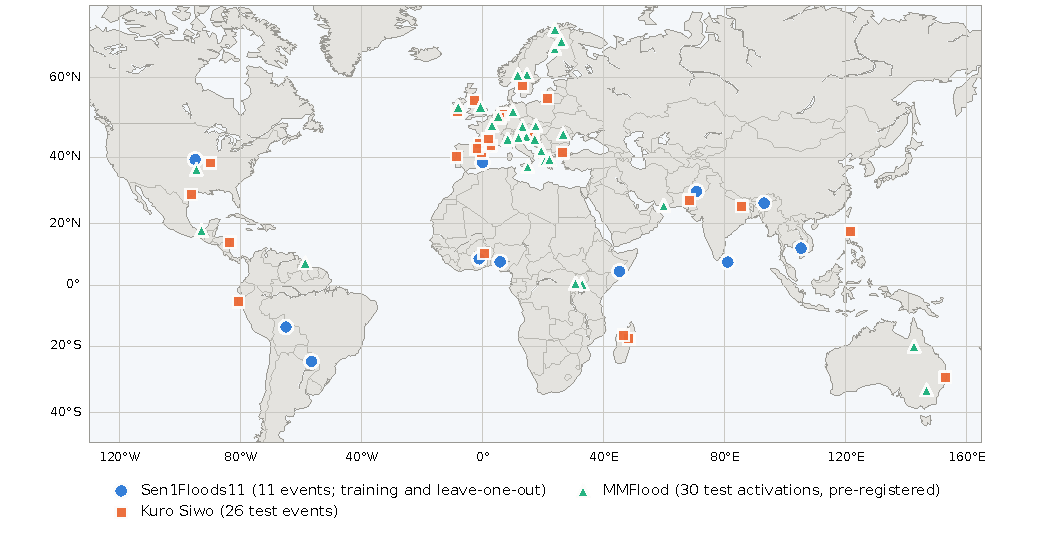
\includegraphics[width=\textwidth]{figures/fig_sites.pdf}
\caption{Locations of the Sen1Floods11 events (centroid of each event's footprint), the 26 Kuro Siwo test events and the 30 MMFlood test activations (activation centre from the MMFlood metadata).}
\label{fig:sites}
\end{figure}

\begin{table}[t]
\caption{Datasets and their role. Events are the statistical unit for every test.}
\label{tab:data}
\centering
\begin{tabular}{llll}
\toprule
Dataset & Events & Chips & Role \\
\midrule
Sen1Floods11 & 11 & 446 & training; leave-one-flood-out test \\
Kuro Siwo & 26 & 1,962 (33 events) & cross-dataset test; choice of the primary method \\
MMFlood & 30 activations (69 folders) & 1,240 & pre-registered final test \\
\bottomrule
\end{tabular}
\end{table}

\subsection{Models and training}
The main model is a five-level U-Net \citep{ronneberger2015unet} with batch normalisation \citep{ioffe2015bn} and 32 base channels, trained from scratch on VV and VH (normalised with Sen1Floods11 training statistics) for 60 epochs on random $256\times256$ crops with flips and rotations, AdamW \citep{loshchilov2019adamw} (learning rate $10^{-3}$, weight decay $10^{-4}$, cosine schedule) and class-weighted cross-entropy. Three models were trained with different seeds. For the leave-one-flood-out test on Sen1Floods11, one model per held-out flood was trained on the other floods. A second backbone, a U-Net with an ImageNet-pretrained \citep{deng2009imagenet} ResNet-34 encoder \citep{he2016resnet,iakubovskii2019smp}, was trained with the same recipe (learning rate $3\times10^{-4}$, three seeds). A variant of it was trained on Sen1Floods11 plus the Kuro Siwo sample, drawing equal numbers of chips from each per epoch.

\subsection{Compared methods}
No adaptation; AdaBN; TENT (batch-norm affine parameters, entropy, Adam $10^{-3}$, 200 steps) \citep{wang2021tent}; plain self-training with an EMA teacher, following \citet{chen2026cimttda}; physics-checked self-training without AdaBN; and AdaBN followed by physics-checked self-training with either fixed thresholds ($-18$\,dB VV, $-25$\,dB VH, relative height and slope) or the adaptive rule above (the proposed method). An Otsu threshold on VV serves as a model-free reference \citep{otsu1979threshold}. All methods use the same models, crops and number of steps.

\subsection{Metrics and statistics}
For each event and method we report IoU of the water class at threshold 0.5 and under the conformal guarantee at $\alpha=0.1, 0.2, 0.3$, the mean and per-event miss rate, the number of events meeting the target, precision, and the false-alarm rate (the share of dry pixels mapped as water). IoU is averaged over the three models per event. Methods are compared with one-sided Wilcoxon signed-rank tests over events \citep{wilcoxon1945,demsar2006}, with Holm correction across the pre-registered hypotheses \citep{holm1979}.

\subsection{Protocol and pre-registration}
The physics check, its thresholds and the combination with AdaBN were developed on Sen1Floods11 and Kuro Siwo; Kuro Siwo therefore served as a development set. Before any MMFlood data were downloaded, we wrote down the primary method (chosen by a fixed rule from the Kuro Siwo results), the preprocessing and exclusion rules, and four hypotheses: the primary method beats TENT (H1) and AdaBN (H2) under the 20\% guarantee, beats no adaptation at threshold 0.5 (H3), and keeps the mean miss rate at or below 0.20 under the 20\% guarantee (H4). After download, and before any result was seen, we fixed the activation (rather than the region folder) as the statistical unit. Experiments with the second backbone were not pre-registered and are reported as exploratory.

%% =====================================================================
\section{Results}
\label{sec:results}

\subsection{Sen1Floods11, leave one flood out}
On held-out Sen1Floods11 floods, the in-domain setting, all methods except TENT lie within 0.03 IoU of each other (Table~\ref{tab:s1f}). AdaBN followed by physics-checked self-training with the fixed rule is highest at 0.5 (0.574); the adaptive rule is 0.013 lower (not significant). Under the 20\% guarantee the two adaptive variants are highest (0.494--0.497, against 0.479 without adaptation). TENT is the weakest at both thresholds. With only 10 calibration floods the guarantee is conservative: the realised mean miss rate at the 20\% target is 0.12--0.13, and IoU drops by about 0.07. Targets below $1/(n+1)\approx0.09$ cannot be met with an informative threshold, because the correction term alone exceeds them (Fig.~\ref{fig:guarantee}b).

\begin{table}[t]
\caption{Sen1Floods11, leave-one-flood-out (11 floods, radar only): mean IoU at threshold 0.5 and under the 20\% miss-rate guarantee.}
\label{tab:s1f}
\centering
\begin{tabular}{lcc}
\toprule
Method & IoU at 0.5 & IoU, 20\% guarantee \\
\midrule
No adaptation & 0.551 & 0.479 \\
TENT & 0.504 & 0.442 \\
Self-training \citep{chen2026cimttda} & 0.550 & 0.486 \\
AdaBN & 0.573 & 0.479 \\
Physics-checked self-training, fixed rule & 0.566 & 0.491 \\
Physics-checked self-training, adaptive rule & 0.556 & 0.497 \\
AdaBN + physics, fixed rule & 0.574 & 0.484 \\
AdaBN + physics, adaptive rule (proposed) & 0.561 & 0.494 \\
\bottomrule
\end{tabular}
\end{table}

\subsection{Kuro Siwo}
The domain gap is large (Table~\ref{tab:ks}): without adaptation the models miss most flood water at 0.5 (IoU 0.186). Calibration alone recovers much of the gap, because the threshold adapts to the new dataset. Plain self-training does not help, and TENT, although strong at 0.5, loses much of its accuracy once a guarantee is imposed (0.576 to 0.467), because its confidence scores are not comparable across floods. The proposed method is best at every level and keeps an IoU of 0.677 under the 20\% guarantee and 0.565 under the 10\% guarantee. The mean miss rate stays at or below the target for every method.

\begin{table}[t]
\caption{Kuro Siwo, 26 unseen events, U-Net trained on Sen1Floods11, radar only: mean IoU over events (mean over three models).}
\label{tab:ks}
\centering
\begin{tabular}{lcccc}
\toprule
Method & 0.5 & 10\% guar. & 20\% guar. & 30\% guar. \\
\midrule
No adaptation & 0.186 & 0.456 & 0.565 & 0.550 \\
Self-training \citep{chen2026cimttda} & 0.174 & 0.360 & 0.457 & 0.490 \\
TENT & 0.576 & 0.327 & 0.467 & 0.576 \\
AdaBN & 0.570 & 0.399 & 0.562 & 0.584 \\
Physics-checked self-training, adaptive & 0.627 & 0.500 & 0.666 & 0.655 \\
AdaBN + physics, fixed rule & 0.668 & 0.528 & 0.662 & 0.648 \\
AdaBN + physics, adaptive rule (proposed) & 0.673 & 0.565 & 0.677 & 0.644 \\
Otsu threshold on VV (no model) & 0.456 & -- & -- & -- \\
\bottomrule
\end{tabular}
\end{table}

Fig.~\ref{fig:guarantee} shows the whole trade-off. For every target between 0.05 and 0.5 the realised mean miss rate on Kuro Siwo stays just below the target for every method (panel c), so the methods differ only in how much accuracy they keep. AdaBN with physics-checked self-training keeps the most at every target (panel a); its advantage is largest at strict targets, where TENT falls furthest behind. With the adaptive rule the proposed method reaches 0.565 IoU at the 10\% target, against 0.456 without adaptation, 0.399 for AdaBN and 0.327 for TENT (Table~\ref{tab:ks}).

Per event (Fig.~\ref{fig:ksevents}), AdaBN with physics-checked self-training (fixed rule) beats AdaBN alone on 22 of 26 events under the 20\% guarantee (mean gain 0.100 IoU) and no adaptation on 24 of 26 (0.097). AdaBN alone occasionally fails badly; on event 567 it misses 88\% of the water while the physics-checked variant misses 10\%. The worst case for the proposed method is event 118, where it misses 83\% of the water; individual floods can still violate the target even when the mean meets it.

The physics check also produces cleaner maps (Table~\ref{tab:prec}). Under the 20\% guarantee, AdaBN with physics-checked self-training has the highest precision (0.758) and the lowest false-alarm rate (2.7\% of dry pixels), against 0.644 and 6.8\% without adaptation and 0.555 and 7.0\% for TENT. At threshold 0.5 the unadapted model is precise but misses 81\% of the water.

\begin{table}[t]
\caption{Kuro Siwo (26 events, three U-Net models, fixed physics rule): mean miss rate, precision and false-alarm rate (share of dry pixels mapped as water) at threshold 0.5 and under the 20\% guarantee.}
\label{tab:prec}
\centering
\begin{tabular}{lcccccc}
\toprule
 & \multicolumn{3}{c}{Threshold 0.5} & \multicolumn{3}{c}{20\% guarantee} \\
\cmidrule(lr){2-4}\cmidrule(lr){5-7}
Method & Miss rate & Precision & False alarms & Miss rate & Precision & False alarms \\
\midrule
No adaptation & 0.806 & 0.844 & 0.3\% & 0.169 & 0.644 & 6.8\% \\
Self-training & 0.818 & 0.867 & 0.3\% & 0.167 & 0.504 & 8.9\% \\
TENT & 0.335 & 0.854 & 1.6\% & 0.176 & 0.555 & 7.0\% \\
AdaBN & 0.177 & 0.674 & 3.9\% & 0.171 & 0.663 & 4.1\% \\
Physics-checked self-training & 0.440 & 0.921 & 0.9\% & 0.172 & 0.699 & 4.4\% \\
AdaBN + physics & 0.201 & 0.793 & 2.1\% & 0.172 & 0.758 & 2.7\% \\
\bottomrule
\end{tabular}
\end{table}

\begin{figure}[t]
\centering
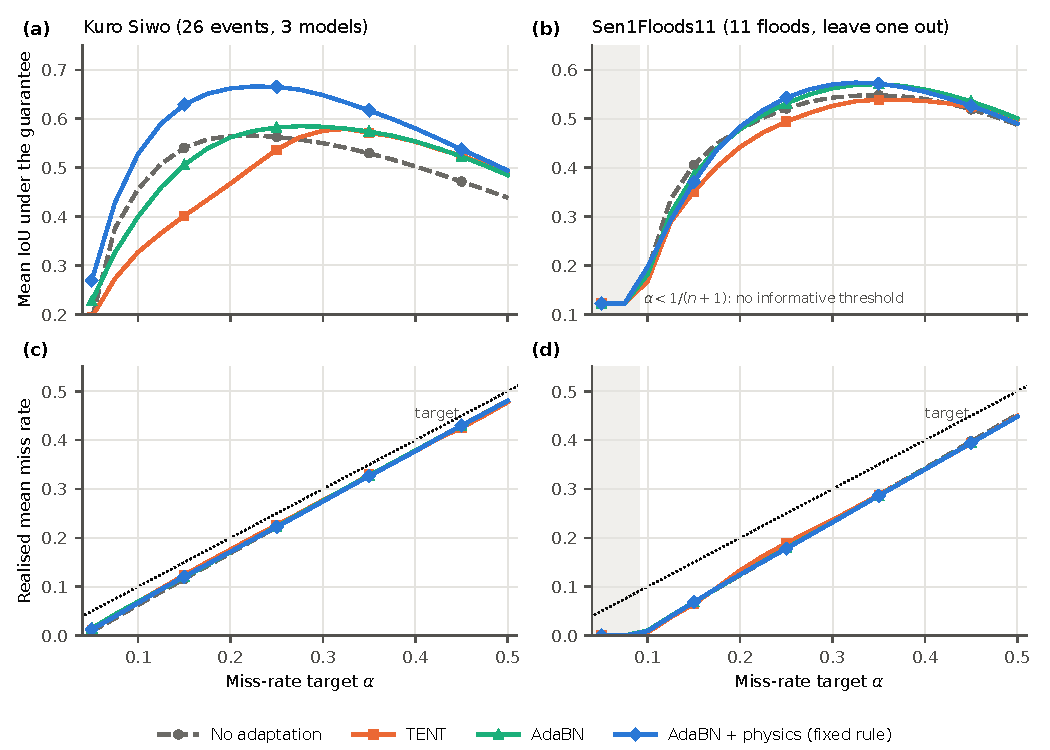
\includegraphics[width=\textwidth]{figures/fig_guarantee.pdf}
\caption{Accuracy and validity of the flood-level guarantee as the miss-rate target $\alpha$ varies. (a, b) Mean IoU under the guarantee; (c, d) realised mean miss rate, with the target as a dotted line. Kuro Siwo: 26 events, mean over three models; Sen1Floods11: 11 floods, leave one flood out. The physics-checked method is shown with the fixed rule, for which histograms are available at every target. Shading in (b, d): targets below $1/(n+1)$ cannot be met with an informative threshold.}
\label{fig:guarantee}
\end{figure}

\begin{figure}[t]
\centering
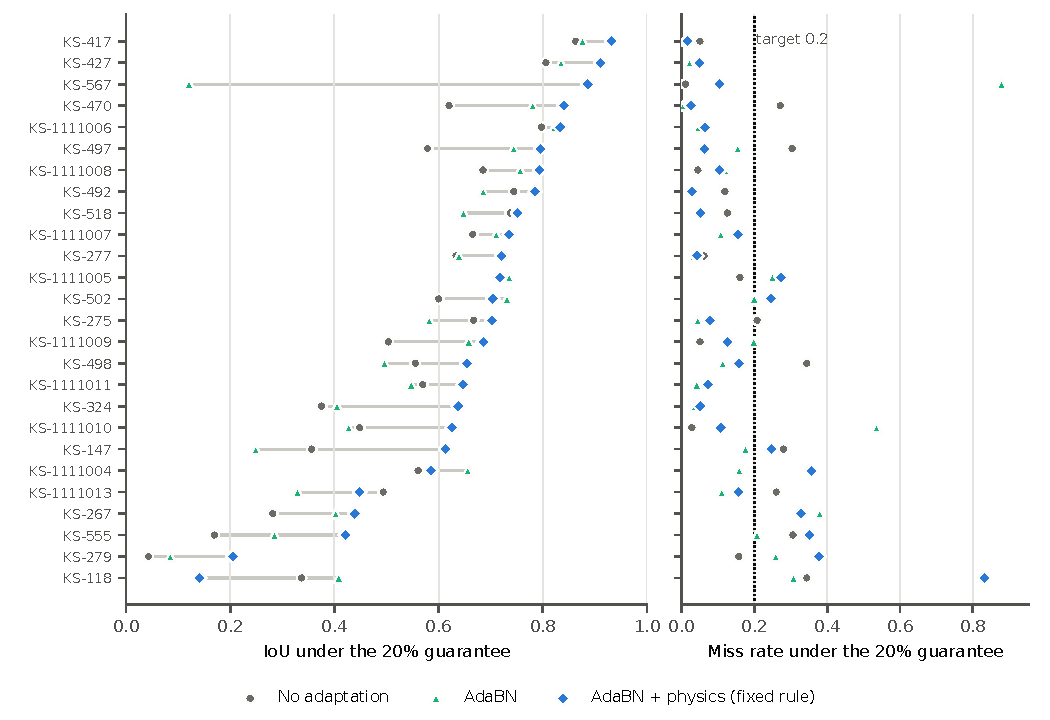
\includegraphics[width=\textwidth]{figures/fig_ks_events.pdf}
\caption{Kuro Siwo, per event, under the 20\% guarantee (mean over three models): IoU (left) and miss rate (right) without adaptation, with AdaBN, and with AdaBN followed by physics-checked self-training (fixed rule). Events are sorted by the IoU of the physics-checked method.}
\label{fig:ksevents}
\end{figure}

Fig.~\ref{fig:maps} shows maps for four Kuro Siwo events, each on the chip with the most labelled water, at the 20\% guarantee threshold. On event 324 the unadapted model and the proposed method map the flooded field cleanly, whereas TENT and AdaBN add false alarms along its edge. On event 1111010, a chip almost entirely under water, TENT misses 90\% of the water while the other methods miss almost none. On event 147 all methods agree. Event 118, where the physics-checked method does worst overall (Fig.~\ref{fig:ksevents}), shows the typical failure: every method misses water in narrow channels and at field margins, and here TENT misses the least (12\% against 26\% for the proposed method).

\begin{figure}[t]
\centering
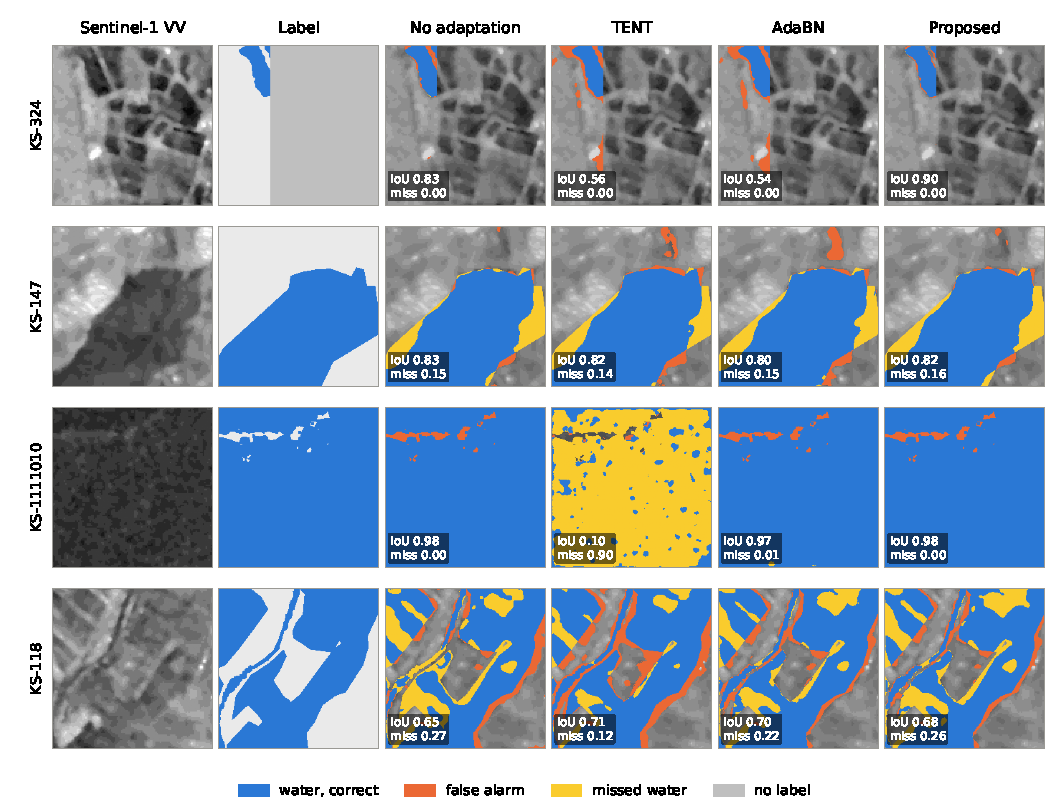
\includegraphics[width=\textwidth]{figures/fig_maps.pdf}
\caption{Example maps on Kuro Siwo (U-Net model seed 0, radar only) at the 20\% guarantee threshold calibrated on the other events. Columns: Sentinel-1 VV (2$\times$2 averaged for display), label, and the maps of each method coloured by agreement with the label; IoU and miss rate refer to the shown chip. Grey label areas are unlabelled and not scored.}
\label{fig:maps}
\end{figure}

\subsection{MMFlood: pre-registered final test}
Table~\ref{tab:mm} reports the primary analysis on 30 activations. H1 and H2 are supported: under the 20\% guarantee the proposed method beats TENT by 0.016 IoU (better on 28 of 30 activations, Holm-corrected $p=4\times10^{-8}$) and AdaBN by 0.014 (28 of 30, $p=6\times10^{-8}$). H3 is not supported: at 0.5 the mean gain over no adaptation is 0.011, but the method is better on only 11 of 30 activations ($p=0.87$); a few large gains (e.g.\ Slovenia, 0.06 to 0.54) raise the mean while most activations are slightly worse. H4 is supported: the mean miss rate under the 20\% guarantee is 0.177. Individual floods vary; about 20 of 30 meet 20\%, and the worst misses 78\%. The analysis with region folders as units gives the same verdicts. Absolute accuracy is low for every method and varies strongly between activations, from 0.01 (Uganda, EMSR438) to 0.54 (Slovenia, EMSR107) at 0.5; we discuss this in Section~\ref{sec:discussion}.

\begin{table}[t]
\caption{MMFlood, pre-registered test, 30 activations (U-Net, three models): mean IoU and miss rate.}
\label{tab:mm}
\centering
\begin{tabular}{lccccc}
\toprule
Method & 0.5 & 10\% guar. & 20\% guar. & 30\% guar. & Miss rate (20\%) \\
\midrule
No adaptation & 0.193 & 0.068 & 0.110 & 0.146 & 0.176 \\
TENT & 0.192 & 0.071 & 0.096 & 0.127 & 0.172 \\
AdaBN & 0.194 & 0.064 & 0.098 & 0.140 & 0.177 \\
AdaBN + physics, fixed rule & 0.211 & 0.079 & 0.111 & 0.158 & 0.176 \\
AdaBN + physics, adaptive rule (proposed) & 0.203 & 0.077 & 0.112 & 0.165 & 0.177 \\
Otsu threshold on VV (no model) & 0.090 & -- & -- & -- & -- \\
\bottomrule
\end{tabular}
\end{table}

\subsection{Second backbone}
With the pretrained ResNet-34 U-Net (exploratory), the unadapted model collapses on Kuro Siwo, predicting almost no water at 0.5 (IoU 0.035). The proposed method recovers an IoU of 0.627 at 0.5 and 0.628 under the 20\% guarantee, against 0.541 for AdaBN, 0.276 for TENT and 0.229 without adaptation, and beats TENT and no adaptation on all 26 events and AdaBN on 19 (Table~\ref{tab:r34}). On MMFlood the same pattern appears as with the U-Net: under the 20\% guarantee the proposed method beats TENT on 30 of 30 activations (Holm-corrected $p=3\times10^{-9}$) and AdaBN on 28 of 30 ($p=4\times10^{-6}$), and at 0.5 it does not beat the unadapted model (11 of 30). TENT is clearly harmful with this backbone (0.053 against 0.109 without adaptation under the guarantee). Adding 33 Kuro Siwo floods to training did not raise MMFlood accuracy (0.207 at 0.5 without adaptation), and the proposed method again beat AdaBN under the guarantee (27 of 30, $p=10^{-4}$). The mean miss rate under the 20\% guarantee was 0.177 for every model and method.

\begin{table}[t]
\caption{Second backbone and more diverse training data (exploratory): mean IoU at 0.5 / under the 20\% guarantee; MMFlood uses activations as units. ``+KS'' denotes training on Sen1Floods11 plus 1,962 Kuro Siwo chips (33 events); Kuro Siwo is then no longer a test set for that model.}
\label{tab:r34}
\centering
\begin{tabular}{lcccc}
\toprule
 & Kuro Siwo (26) & \multicolumn{3}{c}{MMFlood (30 activations)} \\
\cmidrule(lr){2-2}\cmidrule(lr){3-5}
Method & ResNet-34 & U-Net & ResNet-34 & ResNet-34 +KS \\
\midrule
No adaptation & 0.035 / 0.229 & 0.193 / 0.110 & 0.192 / 0.109 & 0.207 / 0.117 \\
TENT & 0.454 / 0.276 & 0.192 / 0.096 & 0.158 / 0.053 & -- \\
AdaBN & 0.560 / 0.541 & 0.194 / 0.098 & 0.198 / 0.104 & 0.204 / 0.106 \\
Proposed & 0.627 / 0.628 & 0.203 / 0.112 & 0.188 / 0.122 & 0.182 / 0.121 \\
\bottomrule
\end{tabular}
\end{table}

\subsection{Sensitivity to the settings}
Table~\ref{tab:sens} changes one setting of the proposed method at a time on Kuro Siwo (model seed 0; for this model AdaBN, TENT and no adaptation reach 0.560, 0.530 and 0.586 IoU under the 20\% guarantee). Under the 20\% guarantee every variant stays between 0.638 and 0.671 IoU, against 0.665 with the defaults, and the mean miss rate stays at 0.170--0.172. The HAND limit hardly matters (3 or 10\,m instead of 5\,m change IoU by at most 0.001), presumably because pixels that pass the darkness and slope tests rarely lie more than a few metres above the drainage network. Moving the dark-threshold caps by 2\,dB or the confidence thresholds to 0.8/0.2 or 0.95/0.05 costs at most 0.011. Fewer self-training steps cost the most (100 steps: $-0.027$), and 400 steps help slightly ($+0.006$). The results therefore do not hinge on a finely tuned setting.

\begin{table}[t]
\caption{Sensitivity of the proposed method (AdaBN + adaptive physics-checked self-training) on Kuro Siwo, U-Net model seed 0, one setting changed at a time from the defaults (caps $-15/-22$\,dB, HAND limit 5\,m, 200 steps, confidence 0.9/0.1): mean IoU at 0.5 and under the guarantee, mean miss rate and events meeting the target under the 20\% guarantee.}
\label{tab:sens}
\centering
\begin{tabular}{lcccccc}
\toprule
Setting & 0.5 & 10\% guar. & 20\% guar. & 30\% guar. & Miss rate & Meeting 20\% \\
\midrule
Defaults & 0.654 & 0.561 & 0.665 & 0.625 & 0.170 & 16/26 \\
Caps $-17/-24$\,dB & 0.655 & 0.543 & 0.659 & 0.625 & 0.170 & 17/26 \\
Caps $-13/-20$\,dB & 0.640 & 0.576 & 0.655 & 0.616 & 0.170 & 16/26 \\
HAND limit 3\,m & 0.655 & 0.561 & 0.665 & 0.626 & 0.170 & 16/26 \\
HAND limit 10\,m & 0.654 & 0.560 & 0.664 & 0.625 & 0.170 & 16/26 \\
100 steps & 0.628 & 0.541 & 0.638 & 0.622 & 0.172 & 15/26 \\
400 steps & 0.671 & 0.571 & 0.671 & 0.628 & 0.170 & 15/26 \\
Confidence 0.8/0.2 & 0.651 & 0.567 & 0.655 & 0.619 & 0.170 & 17/26 \\
Confidence 0.95/0.05 & 0.637 & 0.553 & 0.654 & 0.619 & 0.170 & 15/26 \\
\bottomrule
\end{tabular}
\end{table}

%% =====================================================================
\section{Discussion}
\label{sec:discussion}

\paragraph{The guarantee transfers.} The conformal threshold kept the mean miss rate at or below the target on all three datasets, including MMFlood, which played no part in any design decision. For emergency mapping this is arguably the most useful property: the user chooses how much flood water may be missed on average, and the threshold adapts to the new dataset.

\paragraph{Adaptation can harm, and physics prevents it.} On MMFlood, TENT and AdaBN alone produced worse guaranteed maps than no adaptation (0.096 and 0.098 against 0.110 IoU under the 20\% guarantee). Adding the physics check brought the result back to the unadapted level and gave the best result at the 30\% guarantee. On Kuro Siwo, where the radar shift is larger, the same method was far better than no adaptation. Batch-norm re-estimation removes the calibration shift between datasets, and the terrain-checked pseudo-labels then recover flood water the model still misses; neither part alone came close on Kuro Siwo. The scores of physics-checked models also stay comparable across floods, which is what a single calibrated threshold needs.

\paragraph{Low accuracy on MMFlood.} All methods reach only about 0.2 IoU on MMFlood at 0.5. The Sen1Floods11 models transfer poorly to MMFlood's 20\,m images (upsampled to 10\,m), to its labels drawn from EMS rapid-mapping polygons, and to its many floods under vegetation or in built-up areas, where water is not dark \citep{tsyganskaya2018vegetation,zhao2024urbansarfloods}. Lowering the threshold to meet a miss-rate target then brings many false alarms. Neither a pretrained ResNet-34 backbone nor 33 additional training floods from Kuro Siwo raised MMFlood accuracy (0.19--0.21 IoU at 0.5 for all three models), which suggests that the ceiling is set by the mismatch between MMFlood's images and labels and our single-date radar input rather than by model capacity.

A second reason is the small share of flood water. The median MMFlood activation has 2.5\% of its valid pixels labelled as flood water, against 10.4\% for a Kuro Siwo event and 11.8\% for a Sen1Floods11 event (Fig.~\ref{fig:mmwater}a). With so little water, a false-alarm rate of only 2.5\% of dry pixels already produces about as many false water pixels as there are true ones, and IoU falls accordingly. Across the 30 activations, IoU rises with the water share (Spearman $\rho=0.62$, $p=2\times10^{-4}$; Fig.~\ref{fig:mmwater}b): the 12 activations with less than 2\% water average 0.10 IoU, the 5 with at least 5\% average 0.35. Published MMFlood baselines \citep{montello2022mmflood} report the mean IoU over the flood and background classes for models trained on MMFlood itself, which the dominant background class inflates, so they are not directly comparable to our water-class IoU after a dataset shift. A model-free reference confirms that MMFlood is hard rather than mishandled: an Otsu threshold on VV, fitted per region folder, reaches only 0.090 IoU on average over the 30 activations (median 0.063), less than half of what every network achieves, whereas on Kuro Siwo the same threshold reaches 0.456. The Otsu IoU also follows the water share, from 0.010 in Germany (EMSR261, 0.5\% water) to 0.30 in Finland--Sweden, Albania and Guyana (6--11\% water). We also checked the raw MMFlood files for eight region folders (Table~\ref{tab:mmraw}). The stored backscatter is linear power (median VV between $-12.7$ and $-7.3$\,dB after conversion), the masks contain only 0 and 1, and the same Otsu threshold gives a similar IoU on our resampled 10\,m chips as on the native 20\,m grid (within 0.03 in six folders, higher on the chips in the other two, whose chips contain more of the flooded area), so neither the unit conversion nor the resampling misaligns images and labels. What the check does reveal is that much of the labelled water is not dark: in the median folder only 40\% of labelled water pixels lie below $-15$\,dB in VV, and in Uganda (EMSR438) labelled water is brighter than dry land (median $-5.8$ against $-9.3$\,dB), as expected for flooded vegetation or built-up areas. Such water is invisible to any method that relies on single-date backscatter, including our physics check.

\begin{table}[t]
\caption{MMFlood raw-data check on one image of eight region folders: labelled water share, median VV backscatter of labelled water and of dry land, share of labelled water darker than $-15$\,dB, and IoU of a per-image Otsu threshold on the native 20\,m grid and, with the same threshold, on our 10\,m chips. Backscatter in dB; country codes ISO 3166.}
\label{tab:mmraw}
\centering
\begin{tabular}{lcccccc}
\toprule
Folder & Water & VV water & VV dry & Water $<-15$\,dB & Otsu, 20\,m & Otsu, chips \\
\midrule
EMSR107-5 (SI) & 3.6\% & $-15.7$ & $-8.7$ & 56\% & 0.077 & 0.080 \\
EMSR167-2 (BE) & 1.1\% & $-12.9$ & $-8.8$ & 30\% & 0.021 & 0.006 \\
EMSR184-4 (AU) & 19.8\% & $-19.7$ & $-10.2$ & 78\% & 0.465 & 0.579 \\
EMSR203-3 (US) & 5.8\% & $-13.3$ & $-10.5$ & 35\% & 0.093 & 0.116 \\
EMSR265-14 (FR) & 24.4\% & $-20.0$ & $-9.2$ & 93\% & 0.744 & 0.770 \\
EMSR438-5 (UG) & 2.2\% & $-5.8$ & $-9.3$ & 2\% & 0.002 & 0.001 \\
EMSR479-0 (MX) & 0.3\% & $-10.1$ & $-7.3$ & 13\% & 0.006 & 0.010 \\
EMSR514-0 (GY) & 12.3\% & $-14.4$ & $-12.2$ & 46\% & 0.132 & 0.366 \\
\bottomrule
\end{tabular}
\end{table}

\begin{figure}[t]
\centering
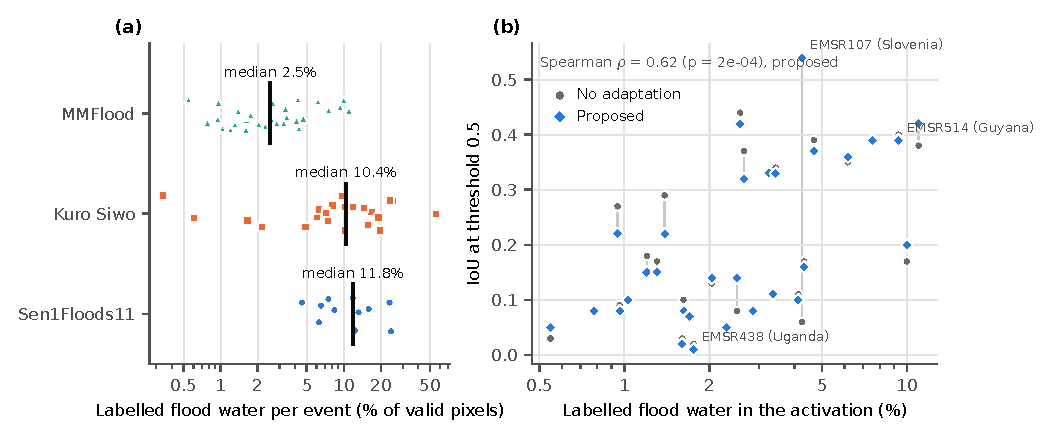
\includegraphics[width=\textwidth]{figures/fig_mmflood_water.pdf}
\caption{(a) Share of valid pixels labelled as flood water, per Sen1Floods11 event, Kuro Siwo event and MMFlood activation (log scale; bar: median). (b) MMFlood: IoU at threshold 0.5 per activation against its water share, without adaptation and with the proposed method (mean over three models).}
\label{fig:mmwater}
\end{figure}

\paragraph{Limitations.} (i) The guarantee bounds the mean miss rate over floods, not the miss rate of each flood; high-probability or per-flood control \citep{bates2021rcps} would need more calibration events. (ii) Calibration needs labelled floods from a similar distribution; across datasets exchangeability may fail \citep{barber2023beyond}. (iii) The dark-water rule cannot detect flooded vegetation or urban flooding. (iv) The adaptive rule and the combination with AdaBN were chosen on Kuro Siwo, so only MMFlood is an untouched test of them. (v) Results use three seeds and one sample of Kuro Siwo. (vi) With $n$ calibration floods, targets below $1/(n+1)$ are unattainable except by mapping everything as water, so strict targets need many calibration floods. (vii) The sensitivity analysis used one model; the settings were robust there, but their interaction was not explored.

%% =====================================================================
\section{Conclusion}
\label{sec:conclusion}
We proposed a label-free test-time adaptation for SAR flood mapping that checks pseudo-labels against radar and terrain physics, and a conformal calibration across flood events that bounds the average miss rate on new floods. Across three datasets, and in a pre-registered final test on MMFlood, the guarantee held, and the physics check made adaptation safe: it beat TENT and batch-norm adaptation under the guarantee and removed the harm that plain adaptation did on MMFlood, although it did not beat the unadapted model there. Future work should strengthen the base models with more diverse training floods and change detection, extend the physics check to flooded vegetation and urban areas, and move from average to per-flood guarantees.

%% =====================================================================
\section*{Declaration of competing interest}
The authors declare that they have no known competing financial interests or personal relationships that could have appeared to influence the work reported in this paper.

\section*{Funding}
This research did not receive any specific grant from funding agencies in the public, commercial, or not-for-profit sectors.

\section*{Data availability}
All datasets used are publicly available: Sen1Floods11 \citep{bonafilia2020sen1floods11}, Kuro Siwo \citep{bountos2024kurosiwo}, MMFlood \citep{montello2022mmflood} and the GLO-30 HAND tiles \citep{glo30hand2022}. The code, the MMFlood exclusion list, the pre-registration text and the stored results behind every table and figure are available at \url{https://github.com/Mahim25800/Research-Flood}.

\section*{Declaration of generative AI and AI-assisted technologies in the manuscript preparation process}
During the preparation of this work the authors used Claude (Anthropic) to assist with code development, running and monitoring the experiments, literature search, preparing figures, drafting and language editing, and formatting the manuscript to the journal template. After using this tool, the authors reviewed and edited the content as needed and take full responsibility for the content of the published article.

\section*{Acknowledgements}
The authors thank the Department of Computer Science, American International University-Bangladesh, for its support.

\section*{CRediT authorship contribution statement}
\textbf{MD Sakib Hasan:} Conceptualization, Data curation, Investigation, Methodology, Resources, Writing -- original draft, Writing -- review \& editing. \textbf{Mostofa Seum:} Conceptualization, Data curation, Investigation, Methodology, Writing -- original draft, Writing -- review \& editing. \textbf{Meer Mursalin:} Data curation, Investigation, Methodology, Visualization, Writing -- review \& editing. \textbf{Tanvir Ahmed:} Project administration, Supervision, Validation, Writing -- review \& editing. \textbf{Rifath Mahmud:} Project administration, Supervision, Validation, Writing -- review \& editing. \textbf{Syeda Anika Tasnim:} Project administration, Supervision, Validation, Writing -- review \& editing.

\bibliographystyle{unsrtnat}
\bibliography{references}

\end{document}
